Utilizando el método de simulación de Montecarlo, se obtiene que, siendo $X$ un variable aleatoria uniforme entre 0 y 1, se puede obtener una distribución exponencial $Y$ dada por la función densidad de probailidad
\begin{equation}
	y(x) = \frac{1}{\lambda} ln\left( \frac{1}{1 - x} \right) \ \ \ \ 0 \leq x \leq 1
\end{equation}

Valiendose de las funciones ``hist'', ``mean'' y ``std'' de Matlab, se asignó arbitrariamente un valor a lambda, en este caso $\lambda = 2$. Además se tomaron 5000 muestras, de forma que se obtuvieron los siguientes resultados:
\begin{figure}[H]
	\centering
	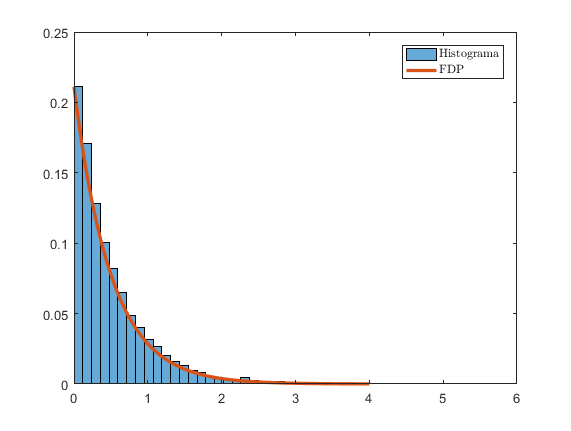
\includegraphics[width=0.7\linewidth]{./ImagenesEjercicio1/Simu-1.png}
	\caption{Iteración del método de Montecarlo.}
	\label{fig:primerit}
\end{figure}

\begin{equation}
\begin{aligned}
		\mu_{Y} = & \ 0.5048 \\
		{\sigma_{Y}}^{2} = & \ 0.2617
\end{aligned}
\end{equation}

Es así que se observa en la Figura (\ref{fig:primerit}) la curva de la f.d.p. teórica sobre el histograma obtenido, confirmando así que se obtuvo realmente una variable aleatoria con la distribución deseada. Además, se desea constatar que los valores de $\mu_{Y}$ y ${\sigma_{Y}}^{2}$, son correctos. Por ser $Y$ una V.A. exponencial, se sabe que $\mu_{Y} = \frac{1}{\lambda}$ y ${\sigma_{Y}}^{2} = \frac{1}{\lambda^2}$, que para el caso presentado son $0.5$ y $0.25$ respectivamente. Si bien los resultados obtenidos no son exactamente iguales, son proximos, siendo el error existente aceptable.  

Bajo las condiciones mencionadas previamente, se realizaron 10 iteracipones más. De esta forma, se obtuvieron los siguientes vores de media y desvio estandar:
\begin{table}[H]
\centering
\begin{tabular}{ccccccccccc}
\hline
\textbf{Iteración}      & \textbf{1} & \textbf{2} & \textbf{3} & \textbf{4} & \textbf{5} & \textbf{6} & \textbf{7} & \textbf{8} & \textbf{9} & \textbf{10} \\ \hline
$\mathbf{\mu}$          & 0,4966     & 0,5015     & 0,5091     & 0,5011     & 0,5095     & 0,4986     & 0,5054     & 0,4856     & 0,4948     & 0,4958      \\
$\mathbf{{\sigma}^{2}}$ & 0,2523     & 0,2548     & 0,2511     & 0,2593     & 0,2600     & 0,2565     & 0,2567     & 0,2373     & 0,2352     & 0,2431     \\ \hline
\end{tabular}
\caption{Iteraciones con valores de media y desvio para la V.A. generada.}
\end{table}

Observando la tabla previa, se repite lo mencionado anteriormente, es decir, que si bien no se obtienen los valores teóricos exactos, estos son proximos a los deseados.

Luego, se realizaron nuevas iteraciones, bajo las mismas especificaciones previas, con el objetivo de presentar en un histograma los distintos valores obtenidos de la media. Es así que luego de 1000 iteraciones se pudo efectuar el siguiente gráfico.
\begin{figure}[H]
	\centering
	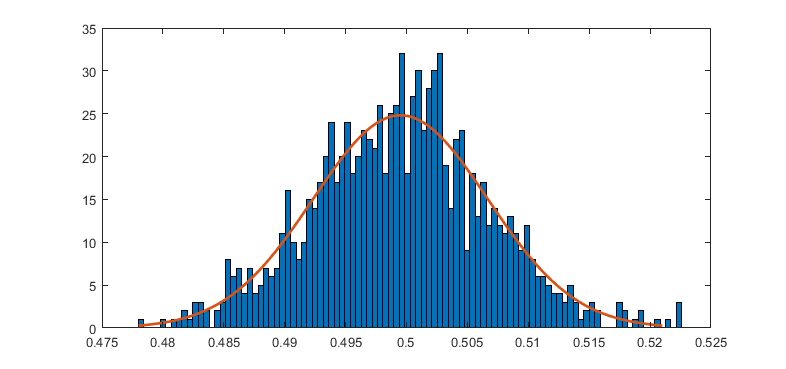
\includegraphics[width=0.8\linewidth]{./ImagenesEjercicio1/Media-1.png}
	\caption{Distribución de la media para 1000 iteraciones.}
	\label{fig:media-mc}
\end{figure}

Se concluye que la media comprende una V.A. gaussiana, con media $\mu = n \cdot \frac{1}{\lambda}$
 y varianza $ \sigma ^2 = n \cdot \frac{1}{\lambda ^2}$. Esto se debe a el teorema central del límite, el cual  indica que, en condiciones muy generales, si Sn es la suma de n
 variables aleatorias independientes y de varianza no nula pero finita, entonces la función de distribución de Sn ,se aproxima bien, a una distribución normal.
  Así pues, el teorema asegura que esto ocurre cuando la suma de
   estas variables aleatorias e independientes es lo suficientemente grande, el cual es nuestro caso.

Finalmente, se desea estimar la cantidad de elementos que se deben generar para estimar la media $\mu_Y$ a través del estimador tal que la probabilidad de que el valor estimado de la media $m_Y$ se aparte más del $6\%$ del valor teórico sea menor al $1\%$, es decir calcular $P\left\lbrace | m_Y - \mu_Y | > \ 0.06 \mu_Y \right\rbrace \leq 0.01$. %Gracias a la desigualdad de Tchebycheff, se puede asegurar que
%\begin{equation}
%	\begin{aligned}
%	\frac{{\sigma_Y}^2}{0.06 \mu_Y} = & \ 0.01
%	\end{aligned}
%\end{equation}
%
%\textcolor{red}{\textbf{MOMENTO... NO ENTIENDO QUE ME PIDE EL PUNTO D... PUTA QUE SAD.}}\\
Por lo tanto, se pide calcular: 
\begin{equation*}
	P\left\lbrace | m_Y - \mu_Y | > \ 0.06 \mu_Y \right\rbrace \leq 0.01
\end{equation*}
\begin{equation*}
	2\cdot P\left\lbrace m_Y - \mu_Y < \ -0.06 \mu_Y \right\rbrace \leq 0.01
\end{equation*}
\begin{equation*}
	P\left\lbrace  \frac{m_Y - \mu_Y}{\sigma_Y}\cdot \sqrt{N} < \ -0.06 \cdot \frac{\mu_Y}{\sigma_Y}\cdot \sqrt{N} \right\rbrace \leq 0.005
\end{equation*}
Siendo $\frac{m_Y - \mu_Y}{\sigma_Y}\cdot \sqrt{N}$ mi nueva V.A. con distribucion normal estándar $\Phi$
\begin{equation*}
\Phi\left( -0.06 \cdot \frac{\mu_Y}{\sigma_Y}\cdot \sqrt{N} \right) \leq 0.005
\end{equation*}

\begin{equation*}
\Phi\left( 0.06 \cdot \frac{\mu_Y}{\sigma_Y}\cdot \sqrt{N} \right) \geq 0.995
\end{equation*}

\begin{equation*}
 0.06 \cdot \frac{\mu_Y}{\sigma_Y}\cdot \sqrt{N} \geq \Phi \left( 0.995 \right)
\end{equation*}
\begin{equation*}
	N \geq \left[ \Phi \left( 0.995 \right) \cdot \frac{\sigma_Y}{\mu_Y \cdot 0.06}\right]^2
\end{equation*}
Sabiendo que $\mu_Y = \frac{1}{\lambda} = \sigma_Y$ y $\Phi \left( 0.995 \right)=2.576$
\begin{equation}
N \geq 1843 
\end{equation}
Finalmente se implementó en código para verificar que esto verifique, como se ve a continuación.

\begin{figure}[H]
	\centering
	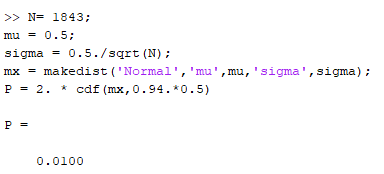
\includegraphics[width=0.4\linewidth]{./ImagenesEjercicio1/implemetacion.PNG}
	\caption{Codigo de verificación en matlab.}
	\label{fig:imple}
\end{figure}